\pagebreak\section{DHT22 Temperature and Humidity Sensor}
\subsection{Experiment URL}
    Use this \href{https://wokwi.com/projects/333082438824624723}{link} to get the \textbf{Wokwi} simulation of this experiment.
    
\subsection{Objectives}
DHT22 is a Humidity and Temperature Sensor, which generates calibrated digital output. DHT22 can be interface with any microcontroller like Arduino, Raspberry Pi, etc. and get instantaneous results. DHT22 is a low cost humidity and temperature sensor which provides high reliability and long term stability.
In this project, we will build a small circuit to interface Arduino with DHT22 Temperature and Humidity Sensor. One of the main applications of connecting DTH22 sensor with Arduino is weather monitoring.

\subsection{Necessary Components}
We will need the following components −
\begin{itemize}
\item 1 x Arduino Uno R3
\item 1 x Breadboard
\item 1 x DHT22 temperature and humidity sensor
\item 1 x 10k $\Omega$ potentiometer
\item 1 x 16x2 LCD screen
\item 1 x USB A-B cable
\item Jumper Wires
\end{itemize}

\subsection{Circuit Diagram}
            \begin{center}
            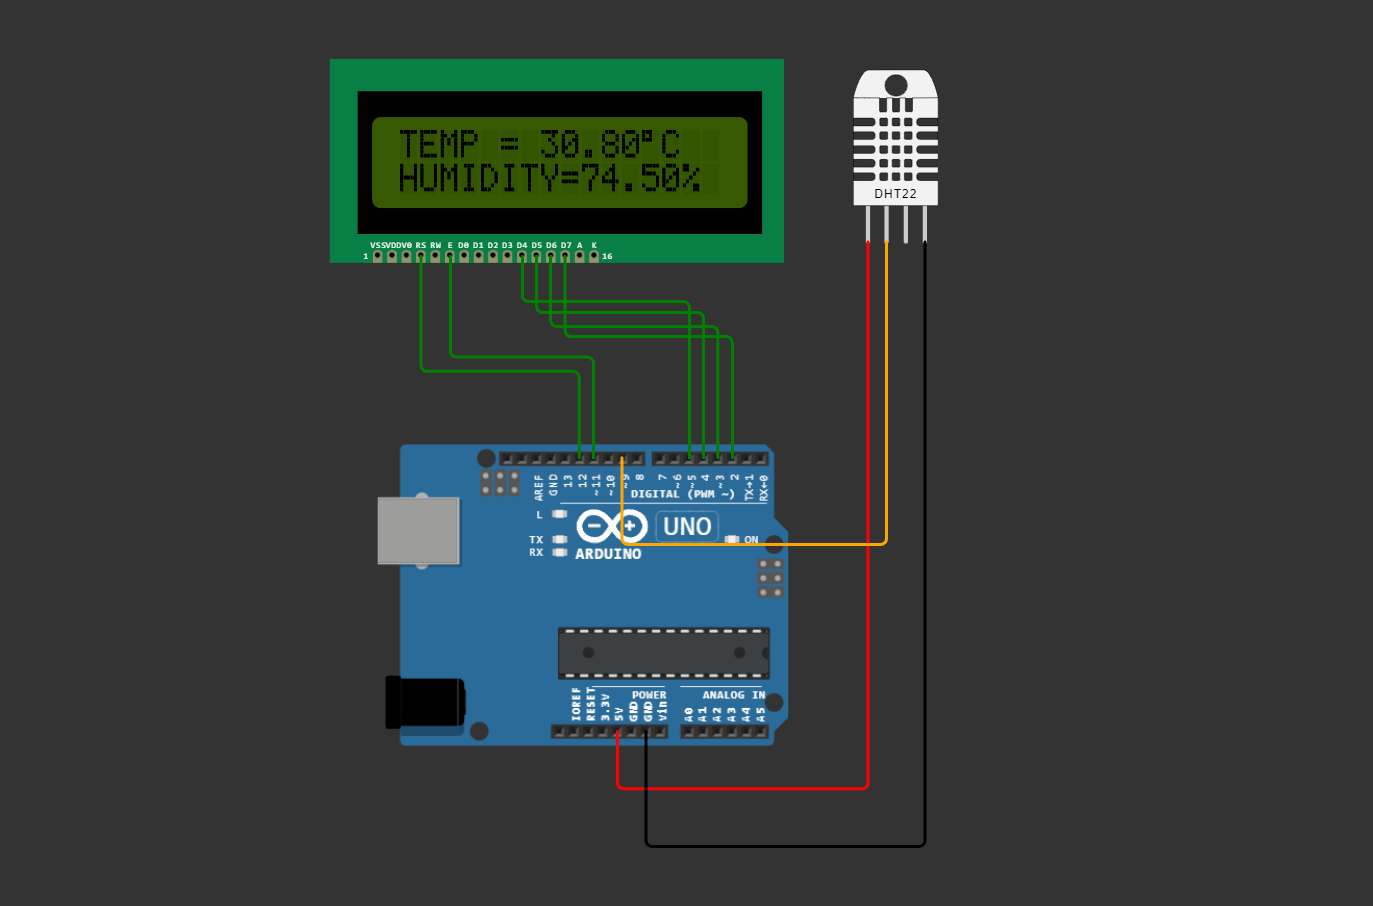
\includegraphics[width =0.7\textwidth]{images/dht22Circuit.png}
            \end{center}

\subsection{Arduino Code}
    \begin{lstlisting}[style = Arduino]
#include <LiquidCrystal.h>
#include <DHT.h>

#define DHTPIN  9
#define DHTTYPE DHT22 


LiquidCrystal lcd(12, 11, 5, 4, 3, 2); // initialize the library with the numbers of the interface pins
DHT dht(DHTPIN, DHTTYPE); //initialize DHT sensor pin


void setup() {
  dht.begin();
  lcd.begin(16, 2); // set up the LCD's number of columns and rows
  
  lcd.setCursor(0,0);

  lcd.print("Initializing....");
  delay(1000);

}

void loop() {
  float temp = dht.readTemperature();
//float tempF = dht.readTemperature(true);
  float hum = dht.readHumidity();

  lcd.clear();
  
  lcd.setCursor(0,1);
  lcd.print("HUMIDITY=");
  lcd.print(hum);            //Displaying humidity
  lcd.print("%");

  lcd.setCursor(0,0);
  lcd.print("TEMP = ");
  lcd.print(temp);            //Displaying temperature in C
  lcd.print((char)223);
  lcd.print("C");
  delay(2000);
}
 
 \end{lstlisting}